\documentclass[14pt]{extbook}
\usepackage{multicol, enumerate, enumitem, hyperref, color, soul, setspace, parskip, fancyhdr} %General Packages
\usepackage{amssymb, amsthm, amsmath, bbm, latexsym, units, mathtools} %Math Packages
\everymath{\displaystyle} %All math in Display Style
% Packages with additional options
\usepackage[headsep=0.5cm,headheight=12pt, left=1 in,right= 1 in,top= 1 in,bottom= 1 in]{geometry}
\usepackage[usenames,dvipsnames]{xcolor}
\usepackage{dashrule}  % Package to use the command below to create lines between items
\newcommand{\litem}[1]{\item#1\hspace*{-1cm}\rule{\textwidth}{0.4pt}}
\pagestyle{fancy}
\lhead{Progress Quiz 4}
\chead{}
\rhead{Version B}
\lfoot{8448-1521}
\cfoot{}
\rfoot{Fall 2020}
\begin{document}

\begin{enumerate}
\litem{
Describe the zero behavior of the zero $x = -6$ of the polynomial below.\[ f(x) = -6(x - 6)^{9}(x + 6)^{14}(x + 3)^{6}(x - 3)^{9} \]\begin{enumerate}[label=\Alph*.]
\begin{multicols}{2}\item 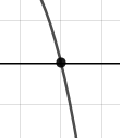
\includegraphics[width = 0.3\textwidth]{../Figures/polyZeroBehaviorCopyAB.png}\item 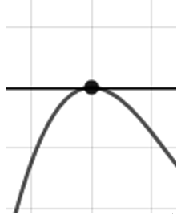
\includegraphics[width = 0.3\textwidth]{../Figures/polyZeroBehaviorCopyBB.png}\item 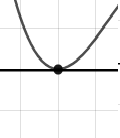
\includegraphics[width = 0.3\textwidth]{../Figures/polyZeroBehaviorCopyCB.png}\item 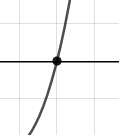
\includegraphics[width = 0.3\textwidth]{../Figures/polyZeroBehaviorCopyDB.png}\end{multicols}\item None of the above.
\end{enumerate} }
\litem{
Which of the following equations \textit{could} be of the graph presented below?
\begin{center}
    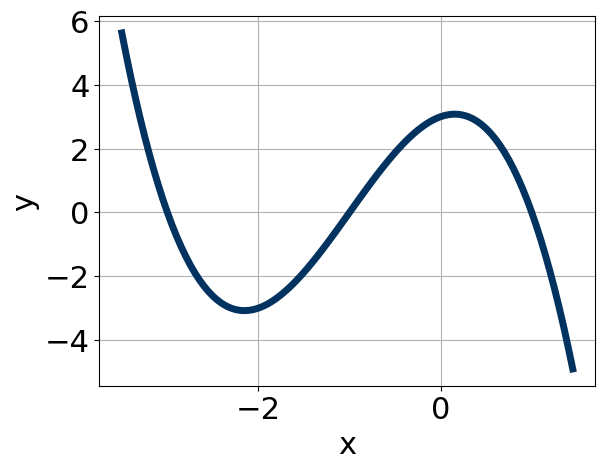
\includegraphics[width=0.5\textwidth]{../Figures/polyGraphToFunctionB.png}
\end{center}
\begin{enumerate}[label=\Alph*.]
\item \( 17(x + 3)^{10} (x - 3)^{8} (x + 2)^{7} \)
\item \( -10(x + 3)^{6} (x - 3)^{7} (x + 2)^{7} \)
\item \( -8(x + 3)^{6} (x - 3)^{9} (x + 2)^{8} \)
\item \( -15(x + 3)^{10} (x - 3)^{6} (x + 2)^{11} \)
\item \( 19(x + 3)^{4} (x - 3)^{6} (x + 2)^{10} \)

\end{enumerate} }
\litem{
Describe the end behavior of the polynomial below.\[ f(x) = 2(x - 9)^{2}(x + 9)^{3}(x - 2)^{4}(x + 2)^{6} \]\begin{enumerate}[label=\Alph*.]
\begin{multicols}{2}\item 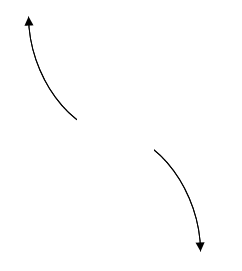
\includegraphics[width = 0.3\textwidth]{../Figures/polyEndBehaviorAB.png}\item 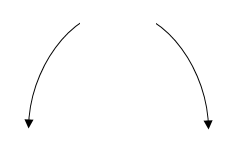
\includegraphics[width = 0.3\textwidth]{../Figures/polyEndBehaviorBB.png}\item 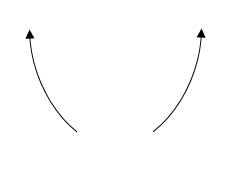
\includegraphics[width = 0.3\textwidth]{../Figures/polyEndBehaviorCB.png}\item 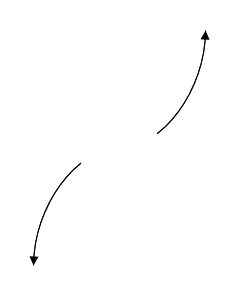
\includegraphics[width = 0.3\textwidth]{../Figures/polyEndBehaviorDB.png}\end{multicols}\item None of the above.
\end{enumerate} }
\litem{
Which of the following equations \textit{could} be of the graph presented below?
\begin{center}
    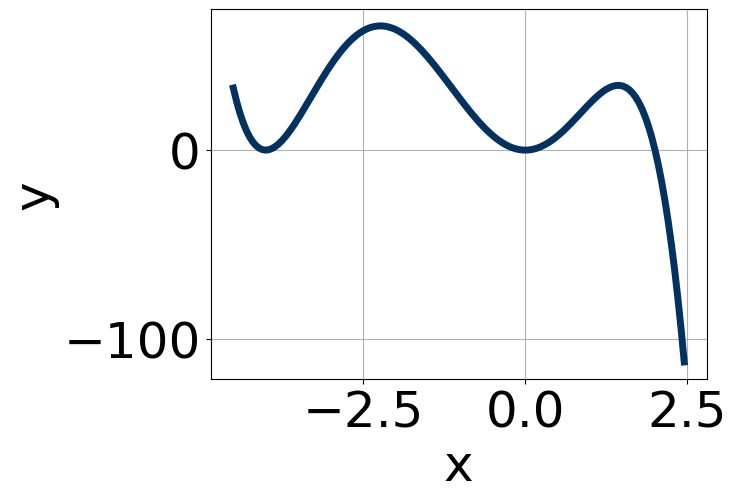
\includegraphics[width=0.5\textwidth]{../Figures/polyGraphToFunctionCopyB.png}
\end{center}
\begin{enumerate}[label=\Alph*.]
\item \( 19x^{5} (x - 2)^{6} (x + 3)^{8} \)
\item \( -15x^{4} (x - 2)^{4} (x + 3)^{11} \)
\item \( 14x^{5} (x - 2)^{10} (x + 3)^{11} \)
\item \( 18x^{5} (x - 2)^{9} (x + 3)^{4} \)
\item \( -15x^{11} (x - 2)^{6} (x + 3)^{5} \)

\end{enumerate} }
\litem{
Describe the end behavior of the polynomial below.\[ f(x) = 6(x - 2)^{4}(x + 2)^{5}(x + 3)^{4}(x - 3)^{4} \]\begin{enumerate}[label=\Alph*.]
\begin{multicols}{2}\item 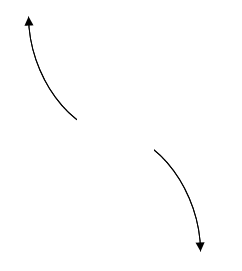
\includegraphics[width = 0.3\textwidth]{../Figures/polyEndBehaviorCopyAB.png}\item 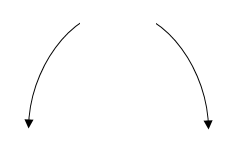
\includegraphics[width = 0.3\textwidth]{../Figures/polyEndBehaviorCopyBB.png}\item 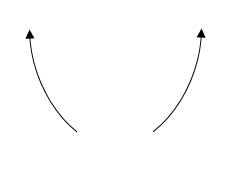
\includegraphics[width = 0.3\textwidth]{../Figures/polyEndBehaviorCopyCB.png}\item 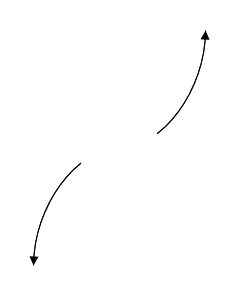
\includegraphics[width = 0.3\textwidth]{../Figures/polyEndBehaviorCopyDB.png}\end{multicols}\item None of the above.
\end{enumerate} }
\litem{
Construct the lowest-degree polynomial given the zeros below. Then, choose the intervals that contain the coefficients of the polynomial in the form $ax^3+bx^2+cx+d$.\[ -7, \frac{2}{3}, \text{ and } -2 \]\begin{enumerate}[label=\Alph*.]
\item \( a \in [-1, 5], b \in [-17.9, -15.3], c \in [-36, -27], \text{ and } d \in [27, 36] \)
\item \( a \in [-1, 5], b \in [23.4, 27.8], c \in [22, 26], \text{ and } d \in [27, 36] \)
\item \( a \in [-1, 5], b \in [-13.7, -11.2], c \in [-60, -51], \text{ and } d \in [-30, -25] \)
\item \( a \in [-1, 5], b \in [23.4, 27.8], c \in [22, 26], \text{ and } d \in [-30, -25] \)
\item \( a \in [-1, 5], b \in [-27.3, -24], c \in [22, 26], \text{ and } d \in [27, 36] \)

\end{enumerate} }
\litem{
Construct the lowest-degree polynomial given the zeros below. Then, choose the intervals that contain the coefficients of the polynomial in the form $ax^3+bx^2+cx+d$.\[ \frac{-3}{2}, -3, \text{ and } \frac{1}{3} \]\begin{enumerate}[label=\Alph*.]
\item \( a \in [2, 7], b \in [24, 32], c \in [16, 21], \text{ and } d \in [-16, -2] \)
\item \( a \in [2, 7], b \in [-25, -22], c \in [16, 21], \text{ and } d \in [6, 10] \)
\item \( a \in [2, 7], b \in [-32, -27], c \in [32, 43], \text{ and } d \in [-16, -2] \)
\item \( a \in [2, 7], b \in [24, 32], c \in [16, 21], \text{ and } d \in [6, 10] \)
\item \( a \in [2, 7], b \in [6, 8], c \in [-30, -29], \text{ and } d \in [6, 10] \)

\end{enumerate} }
\litem{
Construct the lowest-degree polynomial given the zeros below. Then, choose the intervals that contain the coefficients of the polynomial in the form $x^3+bx^2+cx+d$.\[ -5 + 2 i \text{ and } -4 \]\begin{enumerate}[label=\Alph*.]
\item \( b \in [-10, 3], c \in [8, 16], \text{ and } d \in [14, 22] \)
\item \( b \in [8, 18], c \in [62, 78], \text{ and } d \in [116, 124] \)
\item \( b \in [-22, -9], c \in [62, 78], \text{ and } d \in [-118, -111] \)
\item \( b \in [-10, 3], c \in [-2, 3], \text{ and } d \in [-14, -5] \)
\item \( \text{None of the above.} \)

\end{enumerate} }
\litem{
Describe the zero behavior of the zero $x = -4$ of the polynomial below.\[ f(x) = -8(x - 4)^{8}(x + 4)^{11}(x + 9)^{3}(x - 9)^{4} \]\begin{enumerate}[label=\Alph*.]
\begin{multicols}{2}\item 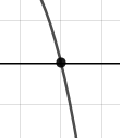
\includegraphics[width = 0.3\textwidth]{../Figures/polyZeroBehaviorAB.png}\item 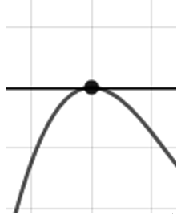
\includegraphics[width = 0.3\textwidth]{../Figures/polyZeroBehaviorBB.png}\item 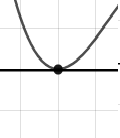
\includegraphics[width = 0.3\textwidth]{../Figures/polyZeroBehaviorCB.png}\item 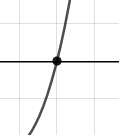
\includegraphics[width = 0.3\textwidth]{../Figures/polyZeroBehaviorDB.png}\end{multicols}\item None of the above.
\end{enumerate} }
\litem{
Construct the lowest-degree polynomial given the zeros below. Then, choose the intervals that contain the coefficients of the polynomial in the form $x^3+bx^2+cx+d$.\[ -5 + 5 i \text{ and } -1 \]\begin{enumerate}[label=\Alph*.]
\item \( b \in [7, 17], c \in [58, 67], \text{ and } d \in [46, 54] \)
\item \( b \in [-15, -6], c \in [58, 67], \text{ and } d \in [-50, -44] \)
\item \( b \in [-4, 5], c \in [4, 7], \text{ and } d \in [1, 6] \)
\item \( b \in [-4, 5], c \in [-10, -3], \text{ and } d \in [-16, 1] \)
\item \( \text{None of the above.} \)

\end{enumerate} }
\end{enumerate}

\end{document}